\documentclass[12pt]{beamer}
\usepackage[utf8]{inputenc}
\usetheme{default}
\usepackage{pgf,pgfarrows,pgfnodes}
\usepackage{graphicx}
\usepackage{algorithmicx} 
\usepackage{color}
\usepackage{lipsum}  
\usepackage{xcolor}
\usepackage{pdfpages}
\usepackage{hyperref}
\usepackage[english]{babel}
\usepackage{graphicx}
\usepackage{ragged2e}
\usepackage{tikz}
\usepackage{media9}
\usepackage{multirow}
\usepackage{tabularx}
\usepackage{array}
\usepackage{mathptmx}       % selects Times Roman as basic font
\usepackage{helvet}         % selects Helvetica as sans-serif font
\usepackage{courier}        % selects Courier as typewriter font
\usepackage{type1cm}        % activate if the above 3 fonts are
\usepackage{textpos} 
\usepackage{pgf,pgfarrows,pgfnodes}
\usepackage{graphicx}
\usepackage{color}
\usepackage{natbib}
\setbeamersize{text margin left=10pt,text margin right=10pt}
\definecolor{idrbt_dark_blue}{HTML}{3333b3}
\definecolor{idrbt_blue}{HTML}{00AEEF} 
\definecolor{adroit_black}{HTML}{222222}
\let\oldcite=\cite                                                              
\renewcommand{\cite}[1]{\textcolor[rgb]{0,.7,0}{\oldcite{#1}}}
\setbeamercolor{item}{fg=idrbt_blue}
\setbeamertemplate{section in toc}
{\leavevmode\leftskip=2ex%
	\llap{%
		\usebeamerfont*{section number projected}%
		\usebeamercolor{section number projected}%
		\begin{pgfpicture}{-1ex}{0ex}{1ex}{2ex}
			\color{idrbt_blue}
			%      \color{red}
			\pgfpathcircle{\pgfpoint{0pt}{.75ex}}{1.7ex}
			\pgfusepath{fill}
			\pgftext[base]{\color{fg}\inserttocsectionnumber}
		\end{pgfpicture}\kern1.25ex%
	}%
	\inserttocsection\par}
\date{}
\title{\textcolor{idrbt_blue}{\rule{112mm}{1.25mm}} \textbf{Lecture-3:\\ Introduction to Beamer}
	 \textcolor{idrbt_blue}{\rule{112mm}{1.25mm}}}
\author{\textcolor{red}{\texttt{\textbf{Manu.V.T.}\\ 
			{\scriptsize Senior Research Fellow\\ Center of Excellence in Cyber Security\\IDRBT}}} }%\newline {\scriptsize Research Fellow} }
%%%%%%%%%%%%%%%%%%%%%%%%%%%%%%%%%%%%%%%%%%%%%%%%%%%%%%%%%%%%%%
\makeatletter
\long\def\beamer@section[#1]#2{%
	\beamer@savemode%
	\mode<all>%
	\ifbeamer@inlecture
	\refstepcounter{section}%
	\beamer@ifempty{#2}%
	{\long\def\secname{#1}\long\def\lastsection{#1}}%
	{\global\advance\beamer@tocsectionnumber by 1\relax%
		\long\def\secname{#2}%
		\long\def\lastsection{#1}%
		\addtocontents{toc}{\protect\beamer@sectionintoc{\the\c@section}{#2\hfill\the\c@page}{\the\c@page}{\the\c@part}%
			{\the\beamer@tocsectionnumber}}}%
	{\let\\=\relax\xdef\sectionlink{{Navigation\the\c@page}{\noexpand\secname}}}%
	\beamer@tempcount=\c@page\advance\beamer@tempcount by -1%
	\beamer@ifempty{#1}{}{%
		\addtocontents{nav}{\protect\headcommand{\protect\sectionentry{\the\c@section}{#1}{\the\c@page}{\secname}{\the\c@part}}}%
		\addtocontents{nav}{\protect\headcommand{\protect\beamer@sectionpages{\the\beamer@sectionstartpage}{\the\beamer@tempcount}}}%
		\addtocontents{nav}{\protect\headcommand{\protect\beamer@subsectionpages{\the\beamer@subsectionstartpage}{\the\beamer@tempcount}}}%
	}%
	\beamer@sectionstartpage=\c@page%
	\beamer@subsectionstartpage=\c@page%
	\def\insertsection{\expandafter\hyperlink\sectionlink}%
	\def\insertsubsection{}%
	\def\insertsubsubsection{}%
	\def\insertsectionhead{\hyperlink{Navigation\the\c@page}{#1}}%
	\def\insertsubsectionhead{}%
	\def\insertsubsubsectionhead{}%
	\def\lastsubsection{}%
	\Hy@writebookmark{\the\c@section}{\secname}{Outline\the\c@part.\the\c@section}{2}{toc}%
	\hyper@anchorstart{Outline\the\c@part.\the\c@section}\hyper@anchorend%
	\beamer@ifempty{#2}{\beamer@atbeginsections}{\beamer@atbeginsection}%
	\fi%
	\beamer@resumemode}%

\def\beamer@subsection[#1]#2{%
	\beamer@savemode%
	\mode<all>%
	\ifbeamer@inlecture%
	\refstepcounter{subsection}%
	\beamer@ifempty{#2}{\long\def\subsecname{#1}\long\def\lastsubsection{#1}}
	{%
		\long\def\subsecname{#2}%
		\long\def\lastsubsection{#1}%
		\addtocontents{toc}{\protect\beamer@subsectionintoc{\the\c@section}{\the\c@subsection}{#2\hfill\the\c@page}{\the\c@page}{\the\c@part}{\the\beamer@tocsectionnumber}}%
	}%
	\beamer@tempcount=\c@page\advance\beamer@tempcount by -1%
	\addtocontents{nav}{%
		\protect\headcommand{\protect\beamer@subsectionentry{\the\c@part}{\the\c@section}{\the\c@subsection}{\the\c@page}{\lastsubsection}}%
		\protect\headcommand{\protect\beamer@subsectionpages{\the\beamer@subsectionstartpage}{\the\beamer@tempcount}}%
	}%
	\beamer@subsectionstartpage=\c@page%
	\edef\subsectionlink{{Navigation\the\c@page}{\noexpand\subsecname}}%
	\def\insertsubsection{\expandafter\hyperlink\subsectionlink}%
	\def\insertsubsubsection{}%
	\def\insertsubsectionhead{\hyperlink{Navigation\the\c@page}{#1}}%
	\def\insertsubsubsectionhead{}%
	\Hy@writebookmark{\the\c@subsection}{#2}{Outline\the\c@part.\the\c@section.\the\c@subsection.\the\c@page}{3}{toc}%
	\hyper@anchorstart{Outline\the\c@part.\the\c@section.\the\c@subsection.\the\c@page}\hyper@anchorend%
	\beamer@ifempty{#2}{\beamer@atbeginsubsections}{\beamer@atbeginsubsection}%
	\fi%
	\beamer@resumemode}

\makeatother
%%%%%%%%%%%%%%%%%%%%%%%%%%%%%%%%%%%%%%%%%%%%%%%%%%%%%%%%%%%%%%
\beamertemplatenavigationsymbolsempty

\addtobeamertemplate{navigation symbols}{}{%
	\usebeamerfont{footline}%
	\usebeamercolor[fg]{footline}%
	\hspace{1em}%
	\insertframenumber/\inserttotalframenumber
}
%%%%%%%%%%%%%%%%%%%%%%%%%%%%%%%%%%%%%%%%%%%%%%%%%%%%%%%%%%%%%%
\begin{document}
	%%%%%%%%%%%%%%%%%%%%%%%%%%%%%%%%%%%%%%%%%%%%%%%%%%%%%%%%%%%%%%%%%%%%%%%%%%%%%%%%%%%%%%%%%%%%%%%%%%%%%%%%%%%%%%%%%%%%%%%%%%%%%
	
	\begin{frame}
	\titlepage
	


\begin{center}
			\begin{tabular}{l>{\centering}p{6.25cm}<{\centering}l}
			\multirow{1}{*}{
\includegraphics[scale=0.15]{./IDRBT_lowres.png}}
			&
         
			&
			\multirow{1}{*}{
\includegraphics[scale=0.2]{./uoh.png}}
		\end{tabular}
\end{center}

\smallskip
	\renewcommand*{\arraystretch}{1.05}



\end{frame}
%%%%%%%%%%%%%%%%%%%%%%%%%%%%%%%%%%%%%%%%%%%%%%%%%%%%%%%%%%%%%%%%%%%%%%%%%%%%%%%%%%%%%%%%%%%%%%%%%%%%%%%%%%%%%%%%%%%%%%%%%%%%%

\begin{frame}
\frametitle{Outline}
\tableofcontents %[hideallsubsections]
\end{frame}
%%%%%%%%%%%%%%%%%%%%%%%%%%%%%%%%%%%%%%%%%%%%%%%%%%%%%%%%%%%%%%%%%%%%%%%%%%%%%%%%%%%%%%%%%%%%%%%%%%%%%%%%%%%%%%%%%%%%%%%%%%%%%

%%%%%%%%%%%%%%%%%%%%%%%%%%%%%%%%%%%%%%%%%%%%%%%%%%%%%%%%%%%%%%%%%%%%%%%%%%%%%%%%%%%%%%%%%%%%%%%%%%%%%%%%%%%%%%%%%%%%%%%%%%%%%
\begin{frame}
\section{Introduction}
\frametitle{Introduction }
	\begin{itemize}\justifying
		\item Beamer is a \LaTeX{} class to create powerful, flexible and nice-looking presentations and slides. 
		\item It enables to make:
		\begin{itemize}
			\item the title page, 
			\item add a logo, 
			\item highlight important points, 
			\item make a table of contents and 
			\item add effects to the presentation
		\end{itemize} 
	\end{itemize}
\end{frame}
%%%%%%%%%%%%%%%%%%%%%%%%%%%%%%%%%%%%%%%%%%%%%%%%%%%%%%%%%%%%%%%%%%%%%%%%%%%%%%%%%%%%%%%%%%%%%%%%%%%%%%%%%%%%%%%%%%%%%%%%%%%%%
%%%%%%%%%%%%%%%%%%%%%%%%%%%%%%%%%%%%%%%%%%%%%%%%%%%%%%%%%%%%%%%%%%%%%%%%%%%%%%%%%%%%%%%%%%%%%%%%%%%%%%%%%%%%%%%%%%%%%%%%%%%%%
\begin{frame}[shrink=20,fragile]
\section{MWE of a simple beamer presentation        }
\frametitle{MWE of a simple beamer presentation}
\begin{verbatim}
	\documentclass{beamer}
	\usepackage[utf8]{inputenc}
 	%%%%%%%%%%%%%%%%%%%%%%%%%%%%%%%%
	\title{A Crash Course on Beamer}
	\author{Manu VT}
	\institute{SCIS@UoH}
	\date{}
 	%%%%%%%%%%%%%%%%%%%%%%%%%%%%%%%%
	\begin{document}
 	%%%%%%%%%%%%%%%%%%%%%%%%%%%%%%%%	
	\frame{\titlepage}
	%%%%%%%%%%%%%%%%%%%%%%%%%%%%%%%%
	\begin{frame}
	\frametitle{Sample frame title}
	This is a text in first frame. 
	\end{frame}
 	%%%%%%%%%%%%%%%%%%%%%%%%%%%%%%%%	
	\end{document}	
\end{verbatim} 
\end{frame}
%%%%%%%%%%%%%%%%%%%%%%%%%%%%%%%%%%%%%%%%%%%%%%%%%%%%%%%%%%%%%%%%%%%%%%%%%%%%%%%%%%%%%%%%%%%%%%%%%%%%%%%%%%%%%%%%%%%%%%%%%%%%%
\begin{frame}%[shrink=20,fragile]
\section{      }
\frametitle{MWE of a simple beamer presentation}
%
\includepdf[pages=1-2]{MWE.pdf}  
\end{frame}
{
	\setbeamercolor{background canvas}{bg=} 
	
\includepdf[pages=1-2]{MWE.pdf}    
}
\begin{frame}[shrink=20,fragile]
\section{Customizing Title Page}
\frametitle{Customizing Title Page}
\begin{verbatim}
\title{Research Methodology in Computer Science}
\subtitle{A Crash Course}
\author{Manu.~V.~T.\inst{1} \and Sitara.~K\inst{2}}
\institute
{
\inst{1}%
IDRBT\\
Hyderabad
\and
\inst{2}%
SCIS\\
University of Hyderabad
}
\date{20/09/2017}
\logo{
\includegraphics[height=1.5cm]{uoh}}
\end{verbatim}
\end{frame}
\begin{frame}[shrink=20,fragile]
\frametitle{Customizing Title Page}

\includegraphics{titlepage}
\end{frame}
%%%%%%%%%%%%%%%%%%%%%%%%%%%%%%%%%%%%%%%%%%%%%%%%%%%%%%%%%%%%%%%%%%%%%%%%%%%%%%%%%%%%%%%%%%%%%%%%%%%%%%%%%%%%%%%%%%%%%%%%%%%%%
\begin{frame}[fragile]
\section{Auto Generation of Table of Contents}
\frametitle{Auto Generation of Table of Contents}
		\begin{verbatim}
			\begin{frame}
			\frametitle{Table of Contents}
			\tableofcontents
			\end{frame}
		\end{verbatim}
\end{frame}
%%%%%%%%%%%%%%%%%%%%%%%%%%%%%%%%%%%%%%%%%%%%%%%%%%%%%%%%%%%%%%%%%%%%%%%%%%%%%%%%%%%%%%%%%%%%%%%%%%%%%%%%%%%%%%%%%%%%%%%%%%%%%
\begin{frame}
\frametitle{Output }

\end{frame}
{
	\setbeamercolor{background canvas}{bg=} 
	
\includepdf[pages=1-4]{toc.pdf}    
}
%%%%%%%%%%%%%%%%%%%%%%%%%%%%%%%%%%%%%%%%%%%%%%%%%%%%%%%%%%%%%%%%%%%%%%%%%%%%%%%%%%%%%%%%%%%%%%%%%%%%%%%%%%%%%%%%%%%%%%%%%%%%%
%%%%%%%%%%%%%%%%%%%%%%%%%%%%%%%%%%%%%%%%%%%%%%%%%%%%%%%%%%%%%%%%%%%%%%%%%%%%%%%%%%%%%%%%%%%%%%%%%%%%%%%%%%%%%%%%%%%%%%%%%%%%%
\begin{frame}[fragile]
\frametitle{Slide Effects}
\begin{verbatim}
	\begin{frame}
	\frametitle{First frame title}
	\section{First frame title}
	This is a text in second frame. 
	For the sake of showing an example.
	
	\begin{itemize}
	\item<1-> Text visible on slide 1
	\item<2-> Text visible on slide 2
	\item<3-> Text visible on slide 3
	\item<4-> Text visible on slide 4
	\end{itemize}
	
	\end{frame}
\end{verbatim}
\end{frame}

\begin{frame}
\frametitle{Slide Effects}

\end{frame}
{
\setbeamercolor{background canvas}{bg=} 

\includepdf[pages=2-5]{effects.pdf}    
}
%%%%%%%%%%%%%%%%%%%%%%%%%%%%%%%%%%%%%%%%%%%%%%%%%%%%%%%%%%%%%%%%%%%%%%%%%%%%%%%%%%%%%%%%%%%%%%%%%%%%%%%%%%%%%%%%%%%%%%%%%%%%%
%%%%%%%%%%%%%%%%%%%%%%%%%%%%%%%%%%%%%%%%%%%%%%%%%%%%%%%%%%%%%%%%%%%%%%%%%%%%%%%%%%%%%%%%%%%%%%%%%%%%%%%%%%%%%%%%%%%%%%%%%%%%%
\begin{frame}[fragile]
\frametitle{Slide Effects with pause command }
\begin{verbatim}
			\begin{frame}
	In this slide \pause
	
	the text will be partially visible \pause
	
	And finally everything will be there
	\end{frame}

\end{verbatim}
\end{frame}
{
\setbeamercolor{background canvas}{bg=} 

\includepdf[pages=2-4]{effects_pause.pdf}    
}
%%%%%%%%%%%%%%%%%%%%%%%%%%%%%%%%%%%%%%%%%%%%%%%%%%%%%%%%%%%%%%%%%%%%%%%%%%%%%%%%%%%%%%%%%%%%%%%%%%%%%%%%%%%%%%%%%%%%%%%%%%%%%
\begin{frame}[fragile]
\section{ Themes and colorthemes }
\frametitle{ Themes and colorthemes }
\begin{verbatim}
\usetheme{Madrid} 
\end{verbatim}
\end{frame}
%%%%%%%%%%%%%%%%%%%%%%%%%%%%%%%%%%%%%%%%%%%%%%%%%%%%%%%%%%%%%%%%%%%%%%%%%%%%%%%%%%%%%%%%%%%%%%%%%%%%%%%%%%%%%%%%%%%%%%%%%%%%%
\begin{frame}[fragile]
\frametitle{ Themes and colorthemes }
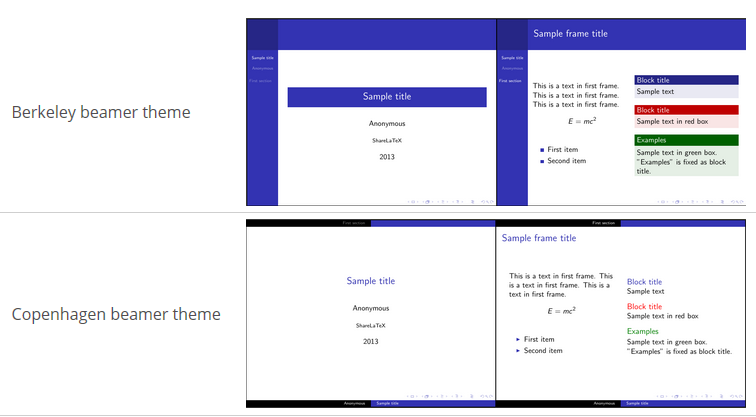
\includegraphics[scale=0.45]{Beamer_Themes_Examples}
\end{frame}
%%%%%%%%%%%%%%%%%%%%%%%%%%%%%%%%%%%%%%%%%%%%%%%%%%%%%%%%%%%%%%%%%%%%%%%%%%%%%%%%%%%%%%%%%%%%%%%%%%%%%%%%%%%%%%%%%%%%%%%%%%%%%%

%%%%%%%%%%%%%%%%%%%%%%%%%%%%%%%%%%%%%%%%%%%%%%%%%%%%%%%%%%%%%%%%%%%%%%%%%%%%%%%%%%%%%%%%%%%%%%%%%%%%%%%%%%%%%%%%%%%%%%%%%%%%%%
\begin{frame}[fragile]
\frametitle{Colorthemes }
\begin{verbatim}


\documentclass{beamer}
\usepackage[utf8]{inputenc}
\usetheme{Madrid}
\usecolortheme{beaver}


\end{verbatim}
\end{frame}
%%%%%%%%%%%%%%%%%%%%%%%%%%%%%%%%%%%%%%%%%%%%%%%%%%%%%%%%%%%%%%%%%%%%%%%%%%%%%%%%%%%%%%%%%%%%%%%%%%%%%%%%%%%%%%%%%%%%%%%%%%%%%%
\begin{frame}[shrink=20,fragile]
\frametitle{Colorthemes }
\begin{verbatim}
	\documentclass{beamer}
	\usepackage[utf8]{inputenc}
	\usetheme{Antibes}
	\usecolortheme{beaver}
	\title{Research Methodology in Computer Science}
	
	\subtitle{A Crash Course}
	
	\author{Manu.~V.~T.\inst{1} \and Sitara.~K\inst{2}}
	
	\institute
	{
	\inst{1}%
	IDRBT\\
	Hyderabad
	\and
	\inst{2}%
	SCIS\\
	University of Hyderabad
	}
	
	\date{20/09/2017}
	
	\logo{
\includegraphics[height=1.5cm]{uoh}}
	
	
	\begin{document}
	\frame{\titlepage}
	\begin{frame}
	\frametitle{Sample frame title}
	
	In this slide, some important text will be
	\alert{highlighted} beause it's important.
	Please, don't abuse it.
	
	\begin{block}{Remark}
	Sample text
	\end{block}
	
	\begin{alertblock}{Important theorem}
	Sample text in red box
	\end{alertblock}
	
	\begin{examples}
	Sample text in green box. "Examples" is fixed as block title.
	\end{examples}
	\end{frame}
	\end{document}	

\end{verbatim}


\end{frame}
\begin{frame}[fragile]
\frametitle{Output }
\end{frame}
{
\setbeamercolor{background canvas}{bg=} 

\includepdf[pages=1-2]{Highlights.pdf}    
}
%%%%%%%%%%%%%%%%%%%%%%%%%%%%%%%%%%%%%%%%%%%%%%%%%%%%%%%%%%%%%%%%%%%%%%%%%%%%%%%%%%%%%%%%%%%%%%%%%%%%%%%%%%%%%%%%%%%%%%%%%%%%%%
\begin{frame}{Video in Slide}
		\includemedia[activate=pageopen,width=122pt,height=90pt,addresource=akiyo_cif.mp4,flashvars={source=akiyo_cif.mp4 &autoPlay=true &loop=true &scaleMode=letterbox}]{}{VPlayer.swf}

	
\end{frame}

\begin{frame}
 \begin{center}
\begin{block}{}
\hspace*{2in}\textbf{\LARGE \textcolor{idrbt_dark_blue}{T}\pause
			    \textcolor{idrbt_blue}{h}\pause
			    \textcolor{idrbt_dark_blue}{a}\pause
			    \textcolor{idrbt_blue}{n}\pause
			    \textcolor{idrbt_dark_blue}{k}\pause
			    \textcolor{idrbt_dark_blue}{Y}\pause
			    \textcolor{idrbt_blue}{o}\pause
			    \textcolor{idrbt_dark_blue}{u} }
\end{block}\end{center}
\end{frame}
\end{document}
%%%%%%%%%%%%%%%%%%%%%%%%%%%%%%%%%%%%%%%%%%%%%%%%%%%%%%%%%%%%%%%%%%%%%%%%%%%%%%%%%%%%%%%%%%%%%%%%%%%%%%%%%%%%%%%%%%%%%%%%%%%%%